\hypertarget{the-ground-robot-world}{%
\section{The Ground Robot World}\label{the-ground-robot-world}}

One of the main differences many see between a vehicle and a robotic
vehicle is whether or not a person is \emph{onboard}. If you are driving
a car, then we would not call this a robot. But if your car was remotely
operated, then some would call it a robotic car.\footnote{The author
  would simply call this a remotely operated car, but either way,
  teleoperation does change how one looks at a vehicle.} Can we make the
robot simulation remotely operated? In this case we mean, \emph{can this
be controlled from an external program?} The answer is yes.

The previous robot code examples allow the user to move a simulated
device around an open rectangle. The world has obstacles and a
simulation should reflect this. So, how should we include obstacles? The
simulation is in two dimensions and so the obstacle will also be in 2D.
The obstacle is then represented as a 2D shape as viewed from above. The
presentation of the simulation is in a window which means at some point
the robot and obstacles are presented on a grid or in a discrete
fashion. This means we have some choices on how to represent the world,
obstacles and other objects, \texttt{fig:enviromodel}.

The environment can be represented in three different manners:
\texttt{continuous}, \texttt{discrete} and \texttt{topological}.
Continuous is how we tend to think about the world. All of the locations
and distances for objects, ourselves and the robots use floating point
values. For example, the center of the robot would be located by a pair
of floating point values and exact information about the robot shape
stored in a database, \texttt{fig:metricmap}.

For a discrete representation, the world is discretized and objects are
located using integer values, \texttt{fig:discretemap}. The world is
then a large checkerboard with a square (pixel) either occupied or not
occupied. Simple two or three color bitmaps then suffice (two for object
maps and optionally a third to track the robot). Painting a pixel white
will indicate that pixel or location is unoccupied. Painting it colored
indicates the pixel is occupied. This approach is known as an
\texttt{occupancy
grid}. The obstacle is simply the collection of black pixels on the
occupancy map. A B/W image file can then be used to generate obstacle
maps. {[}One handy way to accomplish this task is to use a paint program
(or image editing tool) which can export the image into a format that is
easy to read. {]}

\begin{quote}
How one should represent the environment.

\texttt{Continuous\ representation}.

\texttt{Discrete\ representation}.

\texttt{Topological\ representation}.
\end{quote}

Topological representations do not include metric information like the
other two, \texttt{fig:topomap}. Relationships are through graphs that
indicate two things are connected via a path. How they are connected is
another issue. This is very much how humans store maps. You probably
know that to get to your favorite restaurant, you have to pass the Home
Depot and take the next right. Then you keep going until you pass the
Whole Foods market. Then a quick left and there you are. In this
description, no distances were provided and even the notion of left and
right are flexible since we don't require the streets intersect at right
angles.

For the case of the robot simulation, the choice has been partially
made. The robot's world appears as an image which is a discretization or
a grid. Thus we have a discrete environment. We might decide to go with
an obstacle map. Each obstacle is just written into the map and then
disappears in to the large collection of filled pixels. Or we may elect
to keep our obstacles in a continuous representation. However, this
means that translations between the continuous and discrete forms must
happen often.

Continuous and discrete forms each have strengths and weaknesses. We
have very precise information in the continuous form. To increase
precision in the discrete world, we must decrease pixel size which
increases the array storage dramatically or forces a more sophisticated
data format over a simple 2D array. Although storage has increased, many
operations in the discrete world are much easier.

Consider the problem of simulating a robot impact on a object. Say that
the object has an irregular shape. This shape can be approximated by the
pixelized version in the discrete world or by a cubic spline
approximation using a continuous approximation. True that you have much
better accuracy with the cubic spline. The problem is in determining
intersection of the robot boundary with the object boundary. In the
continuous world, we need to take both of the functions and look for
intersecting boundaries at each time step. This requires a complex
nonlinear equation solving routine. {[}Just work out the algebra for two
circles intersecting.{]} For the bitmap version we just check that the
front of the robot is on an occupied pixel or cell (if
cell{[}i{]}{[}j{]} == 1 then ....).

The continuous version will keep objects as objects. For example, if you
have disks that touch, the continuous representation will track the
centers and radii of the two disks. You always know you have multiple
objects. Once converted to a bit map, it could be two adjacent objects
or one connected object or multiple partial objects, etc. It is the
difference between high and low level representations. A topological
representation takes this approach to the next level by removing metric
information and just keeping object description in a connectivity graph.
Many factors enter into the choice of representation. It is always a
trade off between speed, accuracy and simplicity.

\hypertarget{simple-obstacles}{%
\subsection{Simple Obstacles}\label{simple-obstacles}}

The simplest object to study is a disk. It is simple not only in
geometry, but in the more difficult task of determining collision. We
know that if any part of our robot is within a radius of the center, we
have collided. Our robots are round, so collision is just checking the
distance between centers minus the radii. It makes a good stage for a
first path planning exercise. We assume for the moment that our robot
can move freely around the plane (in the open space) and that the plane
is covered with disk shaped obstacles. We also assume that the robot
knows its coordinate location and heading. For a given obstacle map, can
we find a path connecting two points in the plane?

The code to check if two disks intersect is fairly straightforward:

\hypertarget{lst:collisiondetection}{%
\label{lst:collisiondetection}}%
\begin{Shaded}
\begin{Highlighting}[]
\KeywordTok{function}\NormalTok{  collide(center1}\OperatorTok{,}\NormalTok{ r1}\OperatorTok{,}\NormalTok{ center2}\OperatorTok{,}\NormalTok{ r2)}
\NormalTok{    x1 }\OperatorTok{=}\NormalTok{ center1[}\FloatTok{1}\NormalTok{]}
\NormalTok{    y1 }\OperatorTok{=}\NormalTok{ center1[}\FloatTok{2}\NormalTok{]}
\NormalTok{    x2 }\OperatorTok{=}\NormalTok{ center2[}\FloatTok{1}\NormalTok{]}
\NormalTok{    y2 }\OperatorTok{=}\NormalTok{ center2[}\FloatTok{2}\NormalTok{]}
\NormalTok{    d }\OperatorTok{=}\NormalTok{ sqrt((x1}\OperatorTok{{-}}\NormalTok{x2)}\OperatorTok{*}\NormalTok{(x1}\OperatorTok{{-}}\NormalTok{x2) }\OperatorTok{+}\NormalTok{ (y1}\OperatorTok{{-}}\NormalTok{y2)}\OperatorTok{*}\NormalTok{(y1}\OperatorTok{{-}}\NormalTok{y2))}\OperatorTok{{-}}\NormalTok{r1}\OperatorTok{{-}}\NormalTok{r2}
    \KeywordTok{return}\NormalTok{ d}
\KeywordTok{end}
\end{Highlighting}
\end{Shaded}

Where center is a list and r is the radius.\footnote{Keep in mind that
  the robot graphics circle method draws from the bottom of the circle
  and so the center for this formula and the one for the circle method
  need to be adjusted by the radius.}

\begin{quote}
Collision detection with circular robots.
\end{quote}

To check for intersection, we only need to check that \(d\) is small.
Using this we may build a method for a contact sensor. You can treat a
contact sensor as a disk of zero radius and use the formula above
(adjusting for the relation between the center of the robot and the
sensor). Many early robots had sensors placed in a ring around the body
of the robot, \texttt{turtlesensors}. For this example, they will be
contact or touch sensors, but in experimental units often low cost
ultrasonic ranging sensors would be used.

\begin{quote}
A circular robot (like a Create) with touch sensors mounted around the
body.
\end{quote}

Assume that you have a circular robot with a ring of touch or bump
sensors around the body. Knowing the direction of travel, it is possible
to estimate the boundary of the obstacle relative to the robot,
\texttt{turtleboundary}. The boundary normal can be estimated from the
vector created by the sensor location to the robot center. This is a
local estimate only as \texttt{turtleboundary} shows. Being able to
estimate the boundary means that a robot can follow the boundary. The
tangent to the boundary is required for this task.

\begin{figure}
\centering
\includegraphics[width=0.3\textwidth,height=\textheight]{SimulationFigures/turtlecollide2.*}
\caption{Estimating the object boundary.}
\end{figure}

\begin{figure}
\centering
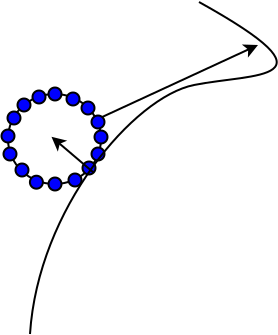
\includegraphics[width=0.3\textwidth,height=\textheight]{SimulationFigures/turtlecollide3.*}
\caption{Bump sensors can only determine the nature of the boundary at
the contact location.}
\end{figure}

Using \texttt{touch\ sensors} to estimate the boundary normal and
tangent.

Using the normal vector, \(\hat{n} = <n_1, n_2>\), the tangent to the
boundary is computed via

\[T = \pm <n_2, -n_1>\]

where the sign is taken so that motion is to the right (right hand
rule). This tangent direction will provide the motion direction for a
boundary following approach. Estimation of the tangent or the direction
of travel can be done with a ring of touch sensors,
\texttt{turtleboundary}.

\hypertarget{using-a-range-sensor}{%
\subsubsection{Using a range sensor}\label{using-a-range-sensor}}

Recall the components in \texttt{fig:intro-components}. There was not a
touch or impact sensor listed. However, there are two types of range
sensors shown. One is a \texttt{LIDAR} and the other is a Kinect. The
next simple planner presented assumes that the robot has a ranging
device. The simplest to model is the LIDAR.

\begin{quote}
Discrete object map.
\end{quote}

A lidar is a simple device conceptually. The unit is able to sweep or
turn in one direction which for our discussion we assume it is
horizontal. It chops up the angular variable into some number of
discrete angles. At each angle or direction, the lidar unit projects a
laser beam out. It receives the reflected signal and computes the
distance. Naively one simply measures the time of flight, divides by two
(for the round trip) and multiplies by \(c\) (the speed of light):
\(D = RT\). This provides the distance of the nearest obstacle at the
current angle. Record the number and move to the next angle.

A sweep creates an array of values where the array index is a function
of the angle and array values are distances. The unit will return the
array. Angles can be reconstructed if you know the starting angle and
the angular increment: \(\theta_i = \theta_0 + i\Delta\theta\). If you
are simulating a given LIDAR unit, then one would use the increment
angle of that unit. If not, then you will decide on the details of
angular increment, maximum range, minimum range and data rate.

How is this done in a discrete environment? Using a two colored image,
let white be free space and red or black indicate occupied space. To
simulate the beam out of the LIDAR, create a virtual line out of the
lidar and follow a straight line along white pixels until you run into a
colored pixel. Stop at the first colored pixel. Using the endpoints of
the line segment (virtual lidar to object pixel), the distance can be
computed. Let \((n,m)\) be the start of the line and let \((i,j)\) be
the location of the object pixel and recall the distance is
\(d = \sqrt{(i-n)^2 + (j-m)^2}\).\footnote{If you wanted an integer
  array you would cast this as an \texttt{int}.}

Any actual lidar unit has an effective range, \(R\). In simulation one
could certainly compute \(d\) as you move out along the ray (or line)
and stop when the max range occurred. This approach will work but it
requires computing the distance function within the innermost loop and
will not result in efficient code. A more effective approach is to just
step out in the radial variable. This means you need to represent the
line or ray in polar coordinates. We will assume that \(R\) is given in
the pixel coordinates and the range would be \(0 \leq r \leq R\). The
other issue is increment value for the lidar simulation. Again, if this
value is taken from an actual unit, then that is the value to use.
Otherwise, at the maximum range, \(R\), we would like that an increment
in the angle selects the ``next'' (adjacent) pixel. So we want
\(\Delta \theta\) to be small enough to hit all the pixels, but no
smaller for performance reasons, see \texttt{inscribedcircle} (b).The
circumference is \(2\pi R\). If a pixel is \(1^2\) units, then we select
\(\Delta\theta \approx 1/(2\pi R)\) (or slightly smaller).

\begin{quote}
Laser angle increments. (a) The first is too small and we resample the
same pixel. (b) The second increment is too large and we miss pixels.
\end{quote}

The lidar simulation algorithm is given in algorithm:
\texttt{Lidar\ Simulation\ \textless{}lidarsim\textgreater{}}

\begin{quote}
\(k=0\)\\
\(\Delta\theta = 1/(2\pi R)\)\\
\textbf{for} \(\theta=0\) to \(2\pi\)\\
\hspace*{0.333em}\hspace*{0.333em}*\emph{for}* \(r=0\) to \(R\)\\
\hspace*{0.333em}\hspace*{0.333em}\hspace*{0.333em}\hspace*{0.333em}i =
(int) \(r \cos \theta\)\\
\hspace*{0.333em}\hspace*{0.333em}\hspace*{0.333em}\hspace*{0.333em}j =
(int) \(r\sin\theta\)\\
\hspace*{0.333em}\hspace*{0.333em}\hspace*{0.333em}\hspace*{0.333em}if
Map(i,j) is occupied then\\
\hspace*{0.333em}\hspace*{0.333em}\hspace*{0.333em}\hspace*{0.333em}\hspace*{0.333em}\hspace*{0.333em}\hspace*{0.333em}\hspace*{0.333em}break
from \(r\) loop\\
\hspace*{0.333em}\hspace*{0.333em}\hspace*{0.333em}\hspace*{0.333em}endif\\
\hspace*{0.333em}\hspace*{0.333em}endfor\\
\hspace*{0.333em}\hspace*{0.333em}dist(k) = \(r\)\\
\hspace*{0.333em}\hspace*{0.333em}k++\\
\hspace*{0.333em}\hspace*{0.333em}\(\theta += \Delta\theta\)\\
endfor
\end{quote}

\textbf{Footnotes}
